\chapter{监督学习}
\section{分类与回归}
监督机器学习问题主要有两种,分别叫作分类(classification)与回归(regression)。

分类问题的目标是预测类别标签(class label),这些标签来自预定义的可选列表。分类问题有时可分为二分类
(binary classification,在两个类别之间进行区分的一种特殊情况)和多分类(multiclass classification,在两个以上的类别之间进行区分)。在二分类问题中,我们通常将其中一个类别称为正类(positive class),另一个类别称为反类(negative class)。这里的“正”并不代表好的方面或正数,而是代表研究对象。

回归任务的目标是预测一个连续值,编程术语叫作浮点数(floating-point number),数学术语叫作实数(real number)。


区分分类任务和回归任务有一个简单方法,就是问一个问题:输出是否具有某种连续性。如果在可能的结果之间具有连续性,那么它就是一个回归问题。

\section{泛化、过拟合与欠拟合}
在监督学习中,我们想要在训练数据上构建模型,然后能够对没见过的新数据(这些新数据与训练集具有相同的特性)做出准确预测。如果一个模型能够对没见过的数据做出准确预测,我们就说它能够从训练集\textbf{泛化}(generalize)到测试集。我们想要构建一个泛化精度尽可能高的模型。

判断一个算法在新数据上表现好坏的唯一度量,就是在测试集上的评估。然而从直觉上看\footnote{在数学上也可以证明这一点。},我们认为简单的模型对新数据的泛化能力更好。因此,我们总想找到最简单的模型。构建一个对现有信息量来说过于复杂的模型,这被称为\textbf{过拟合}(overfitting)。如果你在拟合模型时过分关注训练集的细节,得到了一个在训练集上表现很好、但不能泛化到新数据上的模型,那么就存在过拟合。与之相反,如果你的模型过于简单,那么你可能无法抓住数据的全部内容以及数据中的变化,你的模型甚至在训练集上的表现就很差。选择过于简单的模型被称为\textbf{欠拟合}(underfitting)。

\figures{Trade-off of model complexity against training and test accuracy}
\subsection*{模型复杂度与数据集大小的关系}
需要注意,模型复杂度与训练数据集中输入的变化密切相关:数据集中包含的数据点的变化范围越大,在不发生过拟合的前提下你可以使用的模型就越复杂。通常来说,收集更多的数据点可以有更大的变化范围,所以更大的数据集可以用来构建更复杂的模型。但是,仅复制相同的数据点或收集非常相似的数据是无济于事的。

收集更多数据,适当构建更复杂的模型,对监督学习任务往往特别有用。本书主要关注固定大小的数据集。在现实世界中,你往往能够决定收集多少数据,这可能比模型调参更为有效。永远不要低估更多数据的力量!

\section{监督学习算法}
现在开始介绍最常用的机器学习算法,并解释这些算法如何从数据中学习以及如何预测。我们还会讨论每个模型的复杂度如何变化,并概述每个算法如何构建模型。我们将说明每个算法的优点和缺点,以及它们最适应用于哪类数据。此外还会解释最重要的参数和选项的含义,许多算法都有分类和回归两种形式。

\subsection{一些样本数据集}
我们将使用一些数据集来说明不同的算法。其中一些数据集很小,而且是模拟的,其目的是强调算法的某个特定方面。其他数据集都是现实世界的大型数据集。

\begin{table}
    \centering
    \caption{一些样本数据集}
    \begin{tabular}{cccl}
        \hline
        名称     & 来源 & 特征量            & 用途      \\
        \hline
        forge  & 模拟 & $26\times 2$   & 二分类数据集  \\
        wave   & 模拟 & $40\times 1$   & 回归算法数据集 \\
        cancer & 真实 & $569\times 30$ & 二分类数据集  \\
        boston & 真实 & $506\times 13$ & 回归数据集   \\
        \hline
    \end{tabular}
\end{table}

\figures{Scatter plot of the forge dataset}

\figures{Plot of the wave dataset}
从特征较少的数据集(也叫低维数据集)中得出的结论可能并不适用于特征较多的数据集(也叫高维数据集)。只要你记住这一点,那么在低维数据集上研究算法也是很有启发的。

\begin{tcolorbox}[breakable]
    包含在 scikit-learn 中的数据集通常被保存为 Bunch 对象,里面包含真实数据以及一些数据集信息。关于 Bunch 对象,你只需要知道它与字典很相似,而且还有一个额外的好处,就是你可以用点操作符来访问对象的值(比如用 \verb|bunch.key| 来代替 \verb|bunch['key']|)。
\end{tcolorbox}

对于我们的目的而言,我们需要扩展boston数据集,输入特征不仅包括这 13 个测量结果,还包括这些特征之间的乘积(也叫\textbf{交互项})。换句话说,我们不仅将犯罪率和公路可达性作为特征,还将犯罪率和公路可达性的乘积作为特征。像这样包含导出特征的方法叫作\textbf{特征工程}(feature engineering)。

\subsection{k近邻}
k-NN 算法可以说是最简单的机器学习算法。构建模型只需要保存训练数据集即可。想要对新数据点做出预测,算法会在训练数据集中找到最近的数据点,也就是它的“最近邻”。

\paragraph{k近邻分类} k-NN 算法最简单的版本只考虑一个最近邻,也就是与我们想要预测的数据点最近的训练数据点。预测结果就是这个训练数据点的已知输出。\autoref{Predictions made by the one-nearest-neighbor model on the forge dataset}给出了这种分类方法在 forge 数据集上的应用。

\figures{Predictions made by the one-nearest-neighbor model on the forge dataset}

除了仅考虑最近邻,我还可以考虑任意个(k 个)邻居。这也是 k 近邻算法名字的来历。在考虑多于一个邻居的情况时,我们用“投票法”(voting)来指定标签。将出现次数更多的类别(也就是 k 个近邻中占多数的类别)作为预测结果。

\figures{Predictions made by the three-nearest-neighbors model on the forge dataset}

\paragraph{分析KNeighborsClassifier} 分别将 1 个、3 个和 9 个邻居三种情况的决策边界可视化,见\autoref{Decision boundaries created by the nearest neighbors model}。

\figures{Decision boundaries created by the nearest neighbors model}

从左图可以看出,使用单一邻居绘制的决策边界紧跟着训练数据。随着邻居个数越来越多,决策边界也越来越平滑。更平滑的边界对应更简单的模型。换句话说,使用更少的邻居对应更高的模型复杂度(如\autoref{Trade-off of model complexity against training and test accuracy}右侧所示),而使用更多的邻居对应更低的模型复杂度(如\autoref{Trade-off of model complexity against training and test accuracy}左侧所示)。假如考虑极端情况,即邻居个数等于训练集中所有数据点的个数,那么每个测试点的邻居都完全相同(即所有训练点),所有预测结果也完全相同(即训练集中出现次数最多的类别)。

我们来研究一下能否证实之前讨论过的模型复杂度和泛化能力之间的关系。先将数据集分成训练集和测试集,然后用不同的邻居个数对训练集和测试集的性能进行评估。输出结果见\autoref{Comparison of training and test accuracy}:

\figures{Comparison of training and test accuracy}

注意,由于更少的邻居对应更复杂的模型,所以做了水平翻转。仅考虑单一近邻时,训练集上的预测结果十分完美。但随着邻居个数的增多,模型变得更简单,训练集精度也随之下降。单一邻居时的测试集精度比使用更多邻居时要低,这表示单一近邻的模型过于复杂。与之相反,当考虑 10 个邻居时,模型又过于简单,性能甚至变得更差。最佳性能在中间的某处,邻居个数大约为 6。

\paragraph{k近邻回归}

k 近邻算法还可以用于回归。我们还是先从单一近邻开始,这次使用 wave 数据集。我们添加了 3 个测试数据点,在 x 轴上用绿色五角星表示。利用单一邻居的预测结果就是最近邻的目标值。在\autoref{Comparing predictions made by nearest neighbors regression}中用蓝色五角星表示。

我们还可以用score方法来评估模型,对于回归问题,这一方法返回的是 $R^2$分数。$R^2$分数也叫作决定系数,是回归模型预测的优度度量,位于0到1之间。$R^2$等于1对应完美预测,$R^2$等于0对应常数模型,即总是预测训练集响应(\verb|y_train|)的平均值:


\paragraph{分析KNeighborsRegressor}
对于我们的一维数据集,可以查看所有特征取值对应的预测结果(图\autoref{Comparing predictions made by nearest neighbors regression})。

\figures{Comparing predictions made by nearest neighbors regression}

从图中可以看出,仅使用单一邻居,训练集中的每个点都对预测结果有显著影响,预测结果的图像经过所有数据点。这导致预测结果非常不稳定。考虑更多的邻居之后,预测结果变得更加平滑,但对训练数据的拟合也不好。
\paragraph{优点、缺点和参数}

一般来说,KNeighbors 分类器有 2 个重要参数:邻居个数与数据点之间距离的度量方法。在实践中,使用较小的邻居个数(比如 3 个或 5 个)往往可以得到比较好的结果,但你应该调节这个参数。选择合适的距离度量方法超出了本书的范围。默认使用欧式距离,它在许多情况下的效果都很好。

k-NN 的优点之一就是模型很容易理解,通常不需要过多调节就可以得到不错的性能。在考虑使用更高级的技术之前,尝试此算法是一种很好的基准方法。构建最近邻模型的速度通常很快,但如果训练集很大(特征数很多或者样本数很大),预测速度可能会比较慢。使用 k-NN 算法时,对数据进行预处理是很重要的(见第 3 章)。这一算法对于有很多特征(几百或更多)的数据集往往效果不好,对于大多数特征的大多数取值都为 0 的数据集(所谓的稀疏数据集)来说,这一算法的效果尤其不好。

虽然 k 近邻算法很容易理解,但由于预测速度慢且不能处理具有很多特征的数据集,所以在实践中往往不会用到。

\subsection{线性模型}
线性模型利用输入特征的\textbf{线性函数}(linear function)进行预测

\paragraph{用于回归的线性模型} 对于回归问题,线性模型预测的一般公式如下:
\begin{equation*}
    \hat{y} = w[0] * x[0] + w[1] * x[1] + \cdots + w[p] * x[p] + b
\end{equation*}
这里 $x[0]$ 到 $x[p]$ 表示单个数据点的特征(本例中特征个数为 $p+1$),$w$ 和 $b$ 是学习模型的
参数,$\hat{y}$ 是模型的预测结果。对于单一特征的数据集,公式如下:
\begin{equation*}
    \hat{y} = w[0] * x[0] + b
\end{equation*}

对于有更多特征的数据集,w 包含沿每个特征坐标轴的斜率。或者,你也可以将预测的响应值看作输入特征的加权求和,权重由 w 的元素给出(可以取负值)。

% \figures{Predictions of a linear model on the wave dataset}

\begin{figure}
    \centering
    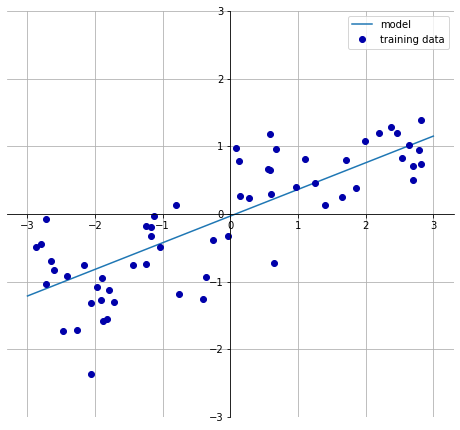
\includegraphics[width=0.6\textwidth]{../Codes/Figures/Predictions of a linear model on the wave dataset.png}
    \caption{Predictions of a linear model on the wave dataset}
    \label{Predictions of a linear model on the wave dataset}
\end{figure}

用于回归的线性模型可以表示为这样的回归模型:对单一特征的预测结果是一条直线,两个特征时是一个平面,或者在更高维度(即更多特征)时是一个超平面。

如果将直线的预测结果与\autoref{Predictions of a linear model on the wave dataset} 中 KNeighborsRegressor 的预测结果进行比较,你会发现直线的预测能力非常受限。似乎数据的所有细节都丢失了。从某种意义上来说,这种说法是正确的。假设目标 y 是特征的线性组合,这是一个非常强的(也有点不现实的)假设。但观察一维数据得出的观点有些片面。对于有多个特征的数据集而言,线性模型可以非常强大。特别地,如果特征数量大于训练数据点的数量,任何目标 y 都可以(在训练集上)用线性函数完美拟合。

\paragraph{线性回归(又名普通最小二乘法)} 线性回归,或者\textbf{普通最小二乘法}(ordinary least squares,OLS),是回归问题最简单也最经典的线性方法。线性回归寻找参数 $w$ 和 $b$,使得对训练集的预测值与真实的回归目标值 $y$ 之间的均方误差最小。\textbf{均方误差}(\emph{mean squared error})是预测值与真实值之差的平方和除以样本数。线性回归没有参数,这是一个优点,但也因此无法控制模型的复杂度。

斜率”参数(w,也叫作权重或系数)被保存在 \verb|coef_| 属性中,而偏移或截距(b)被保存在 \verb|intercept_| 属性中:

\begin{tcolorbox}
    注意到了 \verb|coef_| 和 \verb|intercept_| 结尾处奇怪的下划线。scikit-learn总是将从训练数据中得出的值保存在以下划线结尾的属性中。这是为了将其与用户设置的参数区分开。
\end{tcolorbox}

\verb|intercept_| 属性是一个浮点数,而 \verb|coef_| 属性是一个 NumPy 数组,每个元素对应一个输入特征。由于 wave 数据集中只有一个输入特征,所以 \verb|lr.coef_| 中只有一个元素。

我们来看一下训练集和测试集的性能:
\begin{pyc}
    print('Training set score: {:.2f}'.format(lr.score(X_train, y_train)))
    print('Training set score: {:.2f}'.format(lr.score(X_test, y_test)))
    # 'Training set score: 0.67'
    # 'Training set score: 0.66'
\end{pyc}
$R^2$ 约为 0.66,这个结果不是很好,但我们可以看到,训练集和测试集上的分数非常接近。这说明可能存在欠拟合,而不是过拟合。对于这个一维数据集来说,过拟合的风险很小,因为模型非常简单(或受限)。然而,对于更高维的数据集(即有大量特征的数据集),线性模型将变得更加强大,过拟合的可能性也会变大。

\begin{pyc}
    print('Training set score: {:.2f}'.format(lr.score(X_train, y_train)))
    print('Training set score: {:.2f}'.format(lr.score(X_test, y_test)))
    # Training set score: 0.95
    # Training set score: 0.61
\end{pyc}
训练集和测试集之间的性能差异是过拟合的明显标志,因此我们应该试图找到一个可以控制复杂度的模型。标准线性回归最常用的替代方法之一就是岭回归(ridge regression)

\paragraph{岭回归} 在岭回归中,对系数(w)的选择不仅要在训练数据上得到好的预测结果,而且还要拟合附加约束。我们还希望系数尽量小。换句话说,w 的所有元素都应接近于 0。直观上来看,这意味着每个特征对输出的影响应尽可能小(即斜率很小),同时仍给出很好的预测结果。这种约束是所谓正则化(regularization)的一个例子。正则化是指对模型做显式约束,以避免过拟合。岭回归用到的这种被称为 L2 正则化。
\begin{pyc}
    from sklearn.linear_model import Ridge
    ridge = Ridge().fit(X_train, y_train)
    print('Training set score: {:.2f}'.format(ridge.score(X_train, y_train)))
    print('Training set score: {:.2f}'.format(ridge.score(X_test, y_test)))
    # Training set score: 0.89
    # Training set score: 0.75
\end{pyc}
可以看出,Ridge 在训练集上的分数要低于 LinearRegression,但在测试集上的分数更高。这和我们的预期一致。线性回归对数据存在过拟合。Ridge 是一种约束更强的模型,所以更不容易过拟合。复杂度更小的模型意味着在训练集上的性能更差,但泛化性能更好。由于我们只对泛化性能感兴趣,所以应该选择 Ridge 模型而不是 LinearRegression 模型。

Ridge 模型在模型的简单性(系数都接近于 0)与训练集性能之间做出权衡。简单性和训练集性能二者对于模型的重要程度可以由用户通过设置 alpha 参数来指定。alpha 的最佳设定值取决于用到的具体数据集。增大 alpha 会使得系数更加趋向于 0,从而降低训练集性能,但可能会提高泛化性能。

减小 alpha 可以让系数受到的限制更小,即在\autoref{Trade-off of model complexity against training and test accuracy}中向右移动。对于非常小的 alpha 值,系数几乎没有受到限制,我们得到一个与 LinearRegression 类似的模型。

\figures{Comparing coefficient magnitudes for ridge regression}

我们还可以查看 alpha 取不同值时模型的 \verb|coef_| 属性,从而更加定性地理解 alpha 参数是如何改变模型的。更大的 alpha 表示约束更强的模型,所以我们预计大 alpha 对应的\verb|coef_|元素比小 alpha 对应的 \verb|coef_| 元素要小。这一点可以在\autoref{Comparing coefficient magnitudes for ridge regression}中得到证实。

还有一种方法可以用来理解正则化的影响,就是固定 alpha 值,但改变训练数据量。将模型性能作为数据集大小的函数进行绘图,这样的图像叫作\textbf{学习曲线}。

正如所预计的那样,无论是岭回归还是线性回归,所有数据集大小对应的训练分数都要高于测试分数。由于岭回归是正则化的,因此它的训练分数要整体低于线性回归的训练分数。但岭回归的测试分数要更高,特别是对较小的子数据集。如果少于 400 个数据点,线性回归学不到任何内容。随着模型可用的数据越来越多,两个模型的性能都在提升,最终线性回归的性能追上了岭回归。这里要记住的是,\important{如果有足够多的训练数据,正则化变得不那么重要,并且岭回归和线性回归将具有相同的性能}。 \autoref{}中还有一个有趣之处,就是线性回归的训练性能在下降。\tips{如果添加更多数据,模型将更加难以过拟合或记住所有的数据}。

\paragraph{lasso} 除了 Ridge,还有一种正则化的线性回归是 Lasso。与岭回归相同,使用 lasso 也是约束系数使其接近于 0,但用到的方法不同,叫作 L1 正则化。L1 正则化的结果是,使用 lasso 时某些系数刚好为 0。这说明某些特征被模型完全忽略。这可以看作是一种自动化的特征选择。某些系数刚好为 0,这样模型更容易解释,也可以呈现模型最重要的特征。

如你所见,Lasso 在训练集与测试集上的表现都很差。这表示存在欠拟合,我们发现模型只用到了 105 个特征中的 4 个。与 Ridge 类似,Lasso 也有一个正则化参数 alpha,可以控制系数趋向于 0 的强度。为了降低欠拟合,我们尝试减小 alpha。这么做的同时,我们还需要增加 \verb|max_iter| 的值(运行迭代的最大次数)。

alpha 值变小,我们可以拟合一个更复杂的模型,在训练集和测试集上的表现也更好。模型性能比使用 Ridge 时略好一点,而且我们只用到了 105 个特征中的 33 个。这样模型可能更容易理解。

但如果把alpha设得太小,那么就会消除正则化的效果,并出现过拟合,得到LinearRegression 类似的结果:


\figures{Comparing coefficient magnitudes for lasso regression}

在实践中,在两个模型中一般首选岭回归。但如果特征很多,你认为只有其中几个是重要的,那么选择 Lasso 可能更好。同样,如果你想要一个容易解释的模型,Lasso 可以给出更容易理解的模型,因为它只选择了一部分输入特征。scikit-learn 还提供了 ElasticNet类,结合了 Lasso 和 Ridge 的惩罚项。在实践中,这种结合的效果最好,不过代价是要调节两个参数:一个用于 L1 正则化,一个用于 L2 正则化。

\paragraph{} 首先来看二分类。这时可以利用下面的公式进行预测:
\begin{equation*}
    \hat{y} = w[0] * x[0] + w[1] * x[1] + \cdots + w[p] * x[p] + b > 0
\end{equation*}
这个公式看起来与线性回归的公式非常相似,但我们没有返回特征的加权求和,而是为预测设置了阈值(0)。

对于用于回归的线性模型,输出 $\hat{y}$ 是特征的线性函数,是直线、平面或超平面(对于更高维的数据集)。对于用于分类的线性模型,\textbf{决策边界}是输入的线性函数。换句话说,(二元)线性分类器是利用直线、平面或超平面来分开两个类别的分类器。

学习线性模型有很多种算法。这些算法的区别在于以下两点:
\begin{itemize}
    \item 系数和截距的特定组合对训练数据拟合好坏的度量方法;
    \item 是否使用正则化,以及使用哪种正则化方法。
\end{itemize}

由于数学上的技术原因,不可能调节 w 和 b 使得算法产生的误分类数量最少。对于我们的目的,以及对于许多应用而言,上面第一点(称为损失函数)的选择并不重要。

最常见的两种线性分类算法是 \textbf{Logistic回归}(logistic regression)和\textbf{线性支持向量机}(linear support vector machine,线性 SVM),

\figures{Decision boundaries of a linear SVM and logistic regression}

对于 LogisticRegression 和 LinearSVC, 决定正则化强度的权衡参数叫作C。\important{C值越大,对应的正则化越弱}。换句话说,如果参数 C 值较大,那么 LogisticRegression和LinearSVC 将尽可能将训练集拟合到最好,而如果 C 值较小,那么模型更强调使系数量($bm{w}$)接近于 0。

参数 C 的作用还有另一个有趣之处。\important{较小的 C 值可以让算法尽量适应“大多数”数据点,而较大的 C 值更强调每个数据点都分类正确的重要性}。

\figures{Decision boundaries of a linear SVM for different values of C}

在\autoref{Decision boundaries of a linear SVM for different values of C}中,左图,C 值很小,对应强正则化。大部分属于类别 0 的点都位于底部,大部分属于类别 1 的点都位于顶部。强正则化的模型会选择一条相对水平的线,有两个点分类错误。中间图,C 值稍大,模型更关注两个分类错误的样本,使决策边界的斜率变大。最后,右图,模型的 C 值非常大,使得决策边界的斜率也很大,现在模型对类别 0 中所有点的分类都是正确的。类别 1 中仍有一个点分类错误,这是因为对这个数据集来说,不可能用一条直线将所有点都分类正确。右侧图中的模型尽量使所有点的分类都正确,但可能无法掌握类别的整体分布。换句话说,这个模型很可能过拟合。

与回归的情况类似,用于分类的线性模型在低维空间中看起来可能非常受限,决策边界只能是直线或平面。同样,在高维空间中,用于分类的线性模型变得非常强大,当考虑更多特征时,避免过拟合变得越来越重要。

我们在乳腺癌数据集上详细分析 LogisticRegression:
\begin{pyc}
    # ConvergenceWarning
    logreg = LogisticRegression().fit(X_train, y_train)
    print('Training set score: {:.3f}'.format(logreg.score(X_train, y_train)))
    print('Test set score: {:.3f}'.format(logreg.score(X_test, y_test)))
    # Training set score: 0.946
    # Test set score: 0.965
\end{pyc}

C=1 的默认值给出了相当好的性能,在训练集和测试集上都达到 95\% 的精度。但由于训练集和测试集的性能非常接近,所以模型很可能是欠拟合的。欠拟合的模型可以考虑增加C值来更好的拟合模型。

\begin{pyc}
    # ConvergenceWarning
    logreg100 = LogisticRegression(C=100).fit(X_train, y_train)
    print('Training set score: {:.3f}'.format(logreg100.score(X_train, y_train)))
    print('Test set score: {:.3f}'.format(logreg100.score(X_test, y_test)))
    # Training set score: 0.944
    # Test set score: 0.958
\end{pyc}

我们还可以研究使用正则化更强的模型时会发生什么。设置 $C=0.01$:

\begin{pyc}
    # ConvergenceWarning
    logreg001 = LogisticRegression(C=0.01).fit(X_train, y_train)
    print('Training set score: {:.3f}'.format(logreg001.score(X_train, y_train)))
    print('Test set score: {:.3f}'.format(logreg001.score(X_test, y_test)))
    # Training set score: 0.934
    # Test set score: 0.930
\end{pyc}

\figures{Coefficients learned by logistic regression for different C}

\begin{tcolorbox}
    第 3 个系数那里发现有趣之处,这个系数是“平均周长”(mean perimeter),它的回归系数在不同的正则参数中符号发生了改变。这也说明,对线性模型系数的解释应该始终持保留态度。
\end{tcolorbox}
\paragraph{优点、缺点和参数}
线性模型的主要参数是正则化参数,在回归模型中叫作 alpha,在 LinearSVC 和 Logistic-Regression 中叫作 C。alpha 值较大或 C 值较小,说明模型比较简单。特别是对于回归模型而言,调节这些参数非常重要。通常在对数尺度上对 C 和 alpha 进行搜索。你还需要确定的是用 L1 正则化还是 L2 正则化。如果你假定只有几个特征是真正重要的,那么你应该用L1 正则化,否则应默认使用 L2 正则化。如果模型的可解释性很重要的话,使用 L1 也会有帮助。由于 L1 只用到几个特征,所以更容易解释哪些特征对模型是重要的,以及这些特征的作用。

线性模型的训练速度非常快,预测速度也很快。这种模型可以推广到非常大的数据集,对稀疏数据也很有效。如果你的数据包含数十万甚至上百万个样本,你可能需要研究如何使用 LogisticRegression 和 Ridge 模型的 solver='sag' 选项,在处理大型数据时,这一选项比默认值要更快。其他选项还有 SGDClassifier 类和 SGDRegressor 类,它们对本节介绍的线性模型实现了可扩展性更强的版本。

线性模型的另一个优点在于,利用我们之间见过的用于回归和分类的公式,理解如何进行预测是相对比较容易的。不幸的是,往往并不完全清楚系数为什么是这样的。如果你的数据集中包含高度相关的特征,这一问题尤为突出。在这种情况下,可能很难对系数做出解释。

如果特征数量大于样本数量,线性模型的表现通常都很好。它也常用于非常大的数据集,只是因为训练其他模型并不可行。但在更低维的空间中,其他模型的泛化性能可能更好。

\begin{tcolorbox}[title=方法链]
    scikit-learn 中所有模型的 fit 方法返回的都是 self。

    \verb|logreg = LinearRegression().fit(X_train, y_train)|

    这里我们利用 fit 的返回值(即 self)将训练后的模型赋值给变量 logreg。这种方法调用的拼接(先调用 \verb|__init__|,然后调用 fit)被称为方法链(method chaining)。scikit-learn 中方法链的另一个常见用法是在一行代码中同时 fit 和 predict。

    \begin{pyc}
        logreg = LogisticRegression()
        y_pred = logreg.fit(X_train, y_train).predict(X_test)
    \end{pyc}

    最后,你甚至可以在一行代码中完成模型初始化、拟合和预测:
    \verb|y_pred = LogisticRegression().fit(X_train, y_train).predict(X_test)|

    不过这种非常简短的写法并不完美。一行代码中发生了很多事情,可能会使代码变得难以阅读。此外,拟合后的回归模型也没有保存在任何变量中,所以我们既不能查看它也不能用它来预测其他数据。
\end{tcolorbox}

\subsection{朴素贝叶斯分类器}
朴素贝叶斯分类器是与线性模型非常相似的一种分类器,但它的训练速度往往更快。这种高效率所付出的代价是,朴素贝叶斯模型的泛化能力要比线性分类器(如LogisticRegression 和 LinearSVC)稍差。朴素贝叶斯模型如此高效的原因在于,它通过单独查看每个特征来学习参数,并从每个特征中收集简单的类别统计数据。

scikit-learn 中实现了三种朴素贝叶斯分类器:GaussianNB、BernoulliNB 和 MultinomialNB。GaussianNB 可 应 用 于 任 意 连 续 数 据, 而BernoulliNB 假定输入数据为二分类数据,MultinomialNB 假定输入数据为计数数据。BernoulliNB 和MultinomialNB 主要用于文本数据分类。

\subsection{决策树}
决策树是广泛用于分类和回归任务的模型。本质上,它从一层层的 if/else 问题中进行学习,并得出结论。这一系列问题可以表示为一棵决策树,如图 2-22 所示。

\href{https://scikit-learn.org/stable/modules/generated/sklearn.datasets.make_moons.html}{make\_moons}

\paragraph{构造决策树}

\paragraph{控制决策树的复杂度} 通常来说,构造决策树直到所有叶结点都是纯的叶结点,这会导致模型非常复杂,并且对训练数据高度过拟合。纯叶结点的存在说明这棵树在训练集上的精度是 100\%。训练集中的每个数据点都位于分类正确的叶结点中。

防止过拟合有两种常见的策略:一种是及早停止树的生长,也叫预剪枝(pre-pruning);另一种是先构造树,但随后删除或折叠信息量很少的结点,也叫后剪枝(post-pruning)或剪枝(pruning)。预剪枝的限制条件可能包括限制树的最大深度、限制叶结点的最大数目,或者规定一个结点中数据点的最小数目来防止继续划分。

scikit-learn 的决策树在 DecisionTreeRegressor 类和 DecisionTreeClassifier 类中实现。scikit-learn 只实现了预剪枝,没有实现后剪枝。

\paragraph{分析决策树}

\paragraph{树的特征重要性}

回归树的用法和分析与分类树非常类似。但在将基于树的模型用于回归时,我们想要指出它的一个特殊性质。DecisionTreeRegressor(以及其他所有基于树的回归模型)不能外推(extrapolate),也不能在训练数据范围之外进行预测。

\figures{The tree has no ability to generate new responses}

一旦输入超出了模型训练数据的范围,模型就只能持续预测最后一个已知数据点。树不能在训练数据的范围之外生成“新的”响应。所有基于树的模型都有这个缺点\footnote{实际上,利用基于树的模型可以做出非常好的预测(比如试图预测价格会上涨还是下跌)。这个例子的目的并不是要说明对时间序列来说树是一个不好的模型,而是为了说明树在预测方式上的特殊性质。}。

\paragraph{优点、缺点和参数} 控制决策树模型复杂度的参数是预剪枝参数,它在树完全展开之前停止树的构造。通常来说,选择一种预剪枝策略(设置 \verb|max_depth|、\verb|max_leaf_nodes| 或 \verb|min_samples_leaf|)足以防止过拟合。

与前面讨论过的许多算法相比,决策树有两个优点:一是得到的模型\important{很容易可视化},非专家也很容易理解(至少对于较小的树而言);二是算法完全\important{不受数据缩放的影响}。由于每个特征被单独处理,而且数据的划分也不依赖于缩放,\tips{因此决策树算法不需要特征预处理,比如归一化或标准化。特别是特征的尺度完全不一样时或者二元特征和连续特征同时存在时,决策树的效果很好}。

决策树的主要缺点在于,即使做了预剪枝,它也经常会过拟合,\important{泛化性能很差}。

\subsection{决策树集成}
集成(ensemble)是合并多个机器学习模型来构建更强大模型的方法。
\paragraph{随机森林}
\paragraph{构造随机森林}
\paragraph{分析随机森林}
\paragraph{优点、缺点和参数} 用于回归和分类的随机森林是目前应用最广泛的机器学习方法之一。这种方法非常强大,通常不需要反复调节参数就可以给出很好的结果,也不需要对数据进行缩放。

从本质上看,随机森林拥有决策树的所有优点,同时弥补了决策树的一些缺陷。仍然使用决策树的一个原因是需要决策过程的紧凑表示。基本上不可能对几十棵甚至上百棵树做出详细解释,随机森林中树的深度往往比决策树还要大(因为用到了特征子集)。因此,如果你需要以可视化的方式向非专家总结预测过程,那么选择单棵决策树可能更好。

\begin{tcolorbox}
    你应该记住,随机森林本质上是随机的,设置不同的随机状态(或者不设置 \verb|random_state|参数)可以彻底改变构建的模型。森林中的树越多,它对随机状态选择的鲁棒性就越好。如果你希望结果可以重现,固定 \verb|random_state| 是很重要的。
\end{tcolorbox}


对于维度非常高的稀疏数据(比如文本数据),随机森林的表现往往不是很好。对于这种数据,使用线性模型可能更合适。即使是非常大的数据集,随机森林的表现通常也很好,训练过程很容易并行在功能强大的计算机的多个 CPU 内核上。不过,随机森林需要更大的内存,训练和预测的速度也比线性模型要慢。对一个应用来说,如果时间和内存很重要的话,那么换用线性模型可能更为明智。

需要调节的重要参数有 \verb|n_estimators| 和 \verb|max_features|,可能还包括预剪枝选项(如 \verb|max_depth|)。\verb|n_estimators| 总是越大越好。对更多的树取平均可以降低过拟合,从而得到鲁棒性更好的集成。不过收益是递减的,而且树越多需要的内存也越多,训练时间也越长。常用的经验法则就是“在你的时间 / 内存允许的情况下尽量多”。

\verb|max_features| 决定每棵树的随机性大小,较小的 \verb|max_features| 可以降低过拟合。一般来说,好的经验就是使用默认值:对于分类,默认值是 \verb|max_features=sqrt(n_features)|; 对 于 回 归, 默 认 值 是 \verb|max_features=max_features|。增大 \verb|max_features| 或 \verb|max_leaf_nodes| 有时也可以提高性能。它还可以大大降低用于训练和预测的时间和空间要求。

\paragraph{梯度提升回归树(梯度提升机)} 虽然名字中含有“回归”,但这个模型既可以用于回归也可以用于分类。与随机森林方法不同,梯度提升\notes{采用连续的方式构造树,每棵树都试图纠正前一棵树的错误}。默认情况下,梯度提升回归树中没有随机化,而是用到了\important{强预剪枝}。梯度提升树通常使用深度很小(1到 5 之间)的树,这样模型占用的内存更少,预测速度也更快。

梯度提升背后的主要思想是合并许多简单的模型(在这个语境中叫作\textbf{弱学习器}),比如深度较小的树。每棵树只能对部分数据做出好的预测,因此,添加的树越来越多,可以不断迭代提高性能。

与随机森林相比,它通常对参数设置更为敏感,但如果参数设置正确的话,模型精度更高。

除了预剪枝与集成中树的数量之外,梯度提升的另一个重要参数是 \verb|learning_rate|(学习率),用于控制每棵树纠正前一棵树的错误的强度。较高的学习率意味着每棵树都可以做出较强的修正,这样模型更为复杂。通过增大 \verb|n_estimators| 来向集成中添加更多树,也可以增加模型复杂度,因为模型有更多机会纠正训练集上的错误。

\begin{tcolorbox}
    由于梯度提升和随机森林两种方法在类似的数据上表现得都很好,因此一种常用的方法就是先尝试随机森林,它的鲁棒性很好。如果随机森林效果很好,但预测时间太长,或者机器学习模型精度小数点后第二位的提高也很重要,那么切换成梯度提升通常会有用。
\end{tcolorbox}

想要将梯度提升应用在大规模问题上,可以研究一下 \href{https://xgboost.readthedocs.io/en/stable/#}{xgboost} 包及其 Python 接口
\paragraph{优点、缺点和参数} 梯度提升决策树是监督学习中最强大也最常用的模型之一。其主要缺点是需要仔细调参,而且训练时间可能会比较长。与其他基于树的模型类似,这一算法不需要对数据进行缩放就可以表现得很好,而且也适用于二元特征与连续特征同时存在的数据集。与其他基于树的模型相同,它也通常不适用于高维稀疏数据。

梯度提升树模型的主要参数包括树的数量 \verb|n_estimators| 和学习率 \verb|learning_rate|,后者用于控制每棵树对前一棵树的错误的纠正强度。这两个参数高度相关,因为 \verb|learning_rate| 越低,就需要更多的树来构建具有相似复杂度的模型。随机森林的 \verb|n_estimators| 值总是越大越好,但梯度提升不同,增大 \verb|n_estimators| 会导致模型更加复杂,进而可能导致过拟合。通常的做法是根据时间和内存的预算选择合适的 \verb|n_estimators|,然后对不同的\verb|learning_rate| 进行遍历。

另一个重要参数是 \verb|max_depth|(或 \verb|max_leaf_nodes|),用于降低每棵树的复杂度。梯度提升模型的 \verb|max_depth| 通常都设置得很小,一般不超过 5。

\subsection{核支持向量机}
核支持向量机(kernelized support vector machine, SVM)是可以推广到更复杂模型的扩展,这些模型无法被输入空间的超平面定义。虽然支持向量机可以同时用于分类和回归,但我们只会介绍用于分类的情况,它在 SVC 中实现。类似的概念也适用于支持向量回归,后者在 SVR 中实现。

核支持向量机背后的数学有点复杂,已经超出了本书的范围。你可以阅读 Hastie、Tibshirani 和 Friedman 合著的\href{https://hastie.su.domains/ElemStatLearn/}{《统计学习基础》}一书的第 12 章了解更多细节。
\subsubsection{线性模型与非线性特征}

\subsubsection{核技巧}
这里需要记住的是,向数据表示中添加非线性特征,可以让线性模型变得更强大。但是,通常来说我们并不知道要添加哪些特征,而且添加许多特征的计算开销可能会很大。幸运的是,有一种巧妙的数学技巧,让我们可以在更高维空间中学习分类器,而不用实际计算可能非常大的新的数据表示。这种技巧叫作核技巧(kernel trick),它的原理是直接计算扩展特征表示中数据点之间的距离(更准确地说是内积),而不用实际对扩展进行计算。

对于支持向量机,将数据映射到更高维空间中有两种常用的方法:一种是多项式核,在一定阶数内计算原始特征所有可能的多项式(比如 feature1 ** 2 * feature2 ** 5);另一种是径向基函数(radial basis function,RBF)核,也叫高斯核。高斯核有点难以解释,因为它对应无限维的特征空间。一种对高斯核的解释是它考虑所有阶数的所有可能的多项式,但阶数越高,特征的重要性越小。

\subsubsection{理解SVM}
在训练过程中,\important{SVM 学习每个训练数据点对于表示两个类别之间的决策边界的重要性}。\tips{通常只有一部分训练数据点对于定义决策边界来说很重要:位于类别之间边界上的那些点}。这些点叫作\textbf{支持向量}(support vector),支持向量机正是由此得名。

想要对新样本点进行预测,需要测量它与每个支持向量之间的距离。分类决策是基于它与支持向量之间的距离以及在训练过程中学到的支持向量重要性(保存在 SVC 的 \verb|dual_coef_| 属性中)来做出的。数据点之间的距离由高斯核给出:
\begin{equation*}
    k_{rbf}(x_1, x_2)=exp(-\gamma ||x_1-x_2||^2)
\end{equation*}
这里 $x_1$ 和 $x_2$ 是数据点,$‖x_1 - x_2‖$ 表示欧氏距离,$\gamma$是控制高斯核宽度的参数。

\subsubsection{SVM调参}
\figures{Decision boundaries and support vectors for different settings}

\autoref{Decision boundaries and support vectors for different settings}中,从左到右,我们将参数 gamma 的值从 0.1 增加到 10。gamma 较小,说明高斯核的半径较大,许多点都被看作比较靠近。这一点可以在图中看出:左侧的图决策边界非常平滑,越向右的图决策边界更关注单个点。小的 gamma 值表示决策边界变化很慢,生成的是复杂度较低的模型,而大的 gamma 值则会生成更为复杂的模型。

从上到下,我们将参数 C 的值从 0.1 增加到 1000。与线性模型相同,C 值很小,说明模型非常受限,每个数据点的影响范围都有限。你可以看到,左上角的图中,决策边界看起来几乎是线性的,误分类的点对边界几乎没有任何影响。再看左下角的图,增大 C 之后这些点对模型的影响变大,使得决策边界发生弯曲来将这些点正确分类。

虽然 SVM 的表现通常都很好,但它对参数的设定和数据的缩放非常敏感。特别地,它要求所有特征有相似的变化范围。我们来看一下每个特征的最小值和最大值,它们绘制在对数坐标上(\autoref{Feature ranges for the Breast Cancer dataset})

\figures{Feature ranges for the Breast Cancer dataset}

从\autoref{Feature ranges for the Breast Cancer dataset}中,我们可以确定乳腺癌数据集的特征具有完全不同的数量级。这对其他模型来说(比如线性模型)可能是小问题,但对核 SVM 却有极大影响。

\subsubsection{为SVM预处理数据}
解决这个问题的一种方法就是对每个特征进行缩放,使其大致都位于同一范围。核 SVM常用的缩放方法就是将所有特征缩放到 0 和 1 之间。我们将在\autoref{chapter03}学习如何使用 MinMaxScaler 预处理方法来做到这一点,到时会给出更多细节。

\subsubsection{优点、缺点和参数}
核支持向量机是非常强大的模型,在各种数据集上的表现都很好。SVM 允许决策边界很复杂,即使数据只有几个特征。\notes{它在低维数据和高维数据(即很少特征和很多特征)上的表现都很好,但对样本个数的缩放表现不好}。在有多达 10 000 个样本的数据上运行 SVM可能表现良好,但如果数据量达到 100 000 甚至更大,在运行时间和内存使用方面可能会面临挑战。

SVM 的另一个缺点是,预处理数据和调参都需要非常小心。这也是为什么如今很多应用中用的都是基于树的模型,比如随机森林或梯度提升(需要很少的预处理,甚至不需要预处理)。此外,SVM 模型很难检查,可能很难理解为什么会这么预测,而且也难以将模型向非专家进行解释。

不过 SVM 仍然是值得尝试的,特别是所有特征的测量单位相似(比如都是像素密度)而且范围也差不多时。

核 SVM 的重要参数是正则化参数 C、核的选择以及与核相关的参数。虽然我们主要讲的是RBF 核,但 scikit-learn 中还有其他选择。\important{RBF 核只有一个参数 gamma,它是高斯核宽度的倒数}。gamma 和 C 控制的都是模型复杂度,较大的值都对应更为复杂的模型。因此,这两个参数的设定通常是强烈相关的,\tips{应该同时调节}。

\subsection{神经网络(深度学习)}
虽然深度学习在许多机器学习应用中都有巨大的潜力,但深度学习算法往往经过精确调整,只适用于特定的使用场景。这里只讨论一些相对简单的方法,即用于分类和回归的\textbf{多层感知机}(multilayer perceptron,MLP),它可以作为研究更复杂的深度学习方法的起点。MLP 也被称为(普通)前馈神经网络,有时也简称为神经网络。

\subsubsection{神经网络模型}
MLP 可以被视为广义的线性模型(GLM),执行多层处理后得到结论。线性回归的预测公式简单来说,$\hat{y}$是输入特征 $x[0]$ 到 $x[p]$ 的加权求和,权重为学到的系数 $w[0]$ 到 $w[p]$。我们可以将这个公式可视化,

\begin{figure}[h]
    \centering
    \begin{tabular}{cc}
        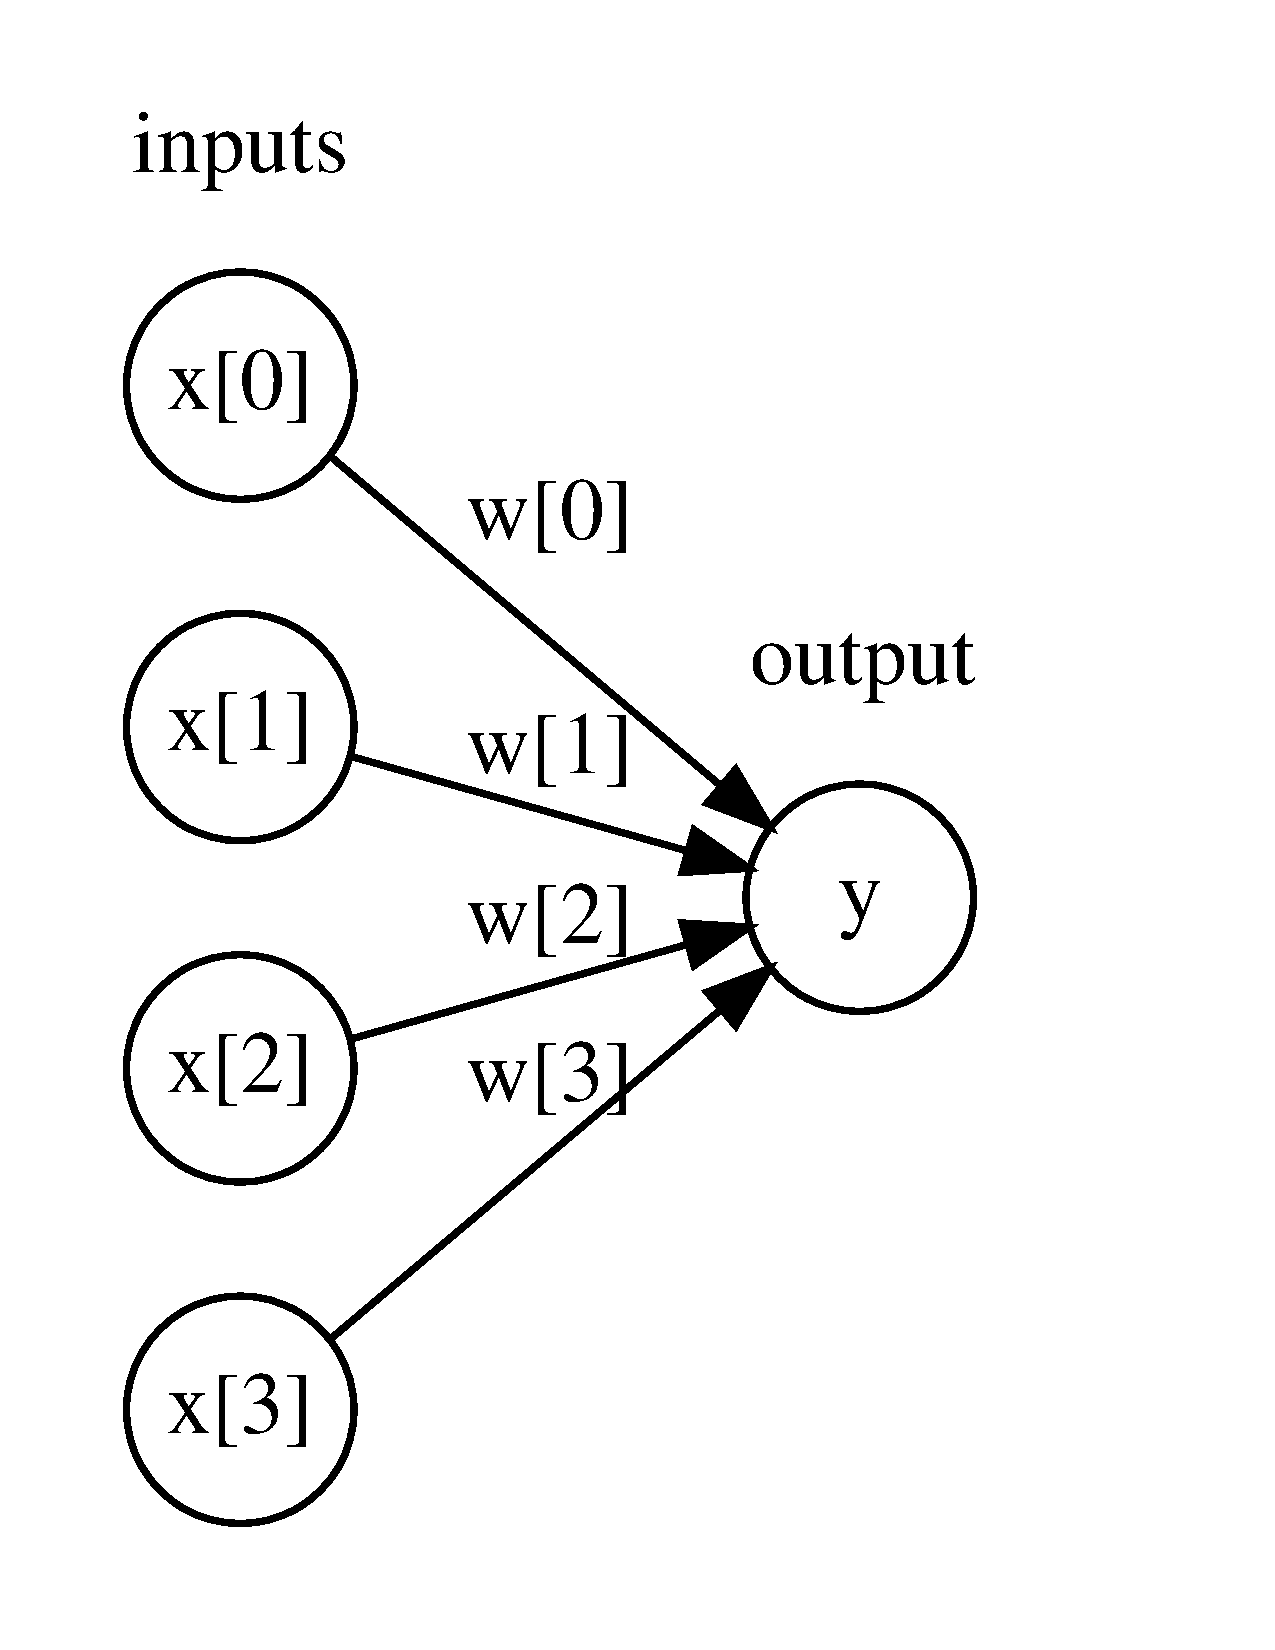
\includegraphics[page=1,width=.45\textwidth]{../Codes/Figures/Visualization of logistic regression.pdf} &
        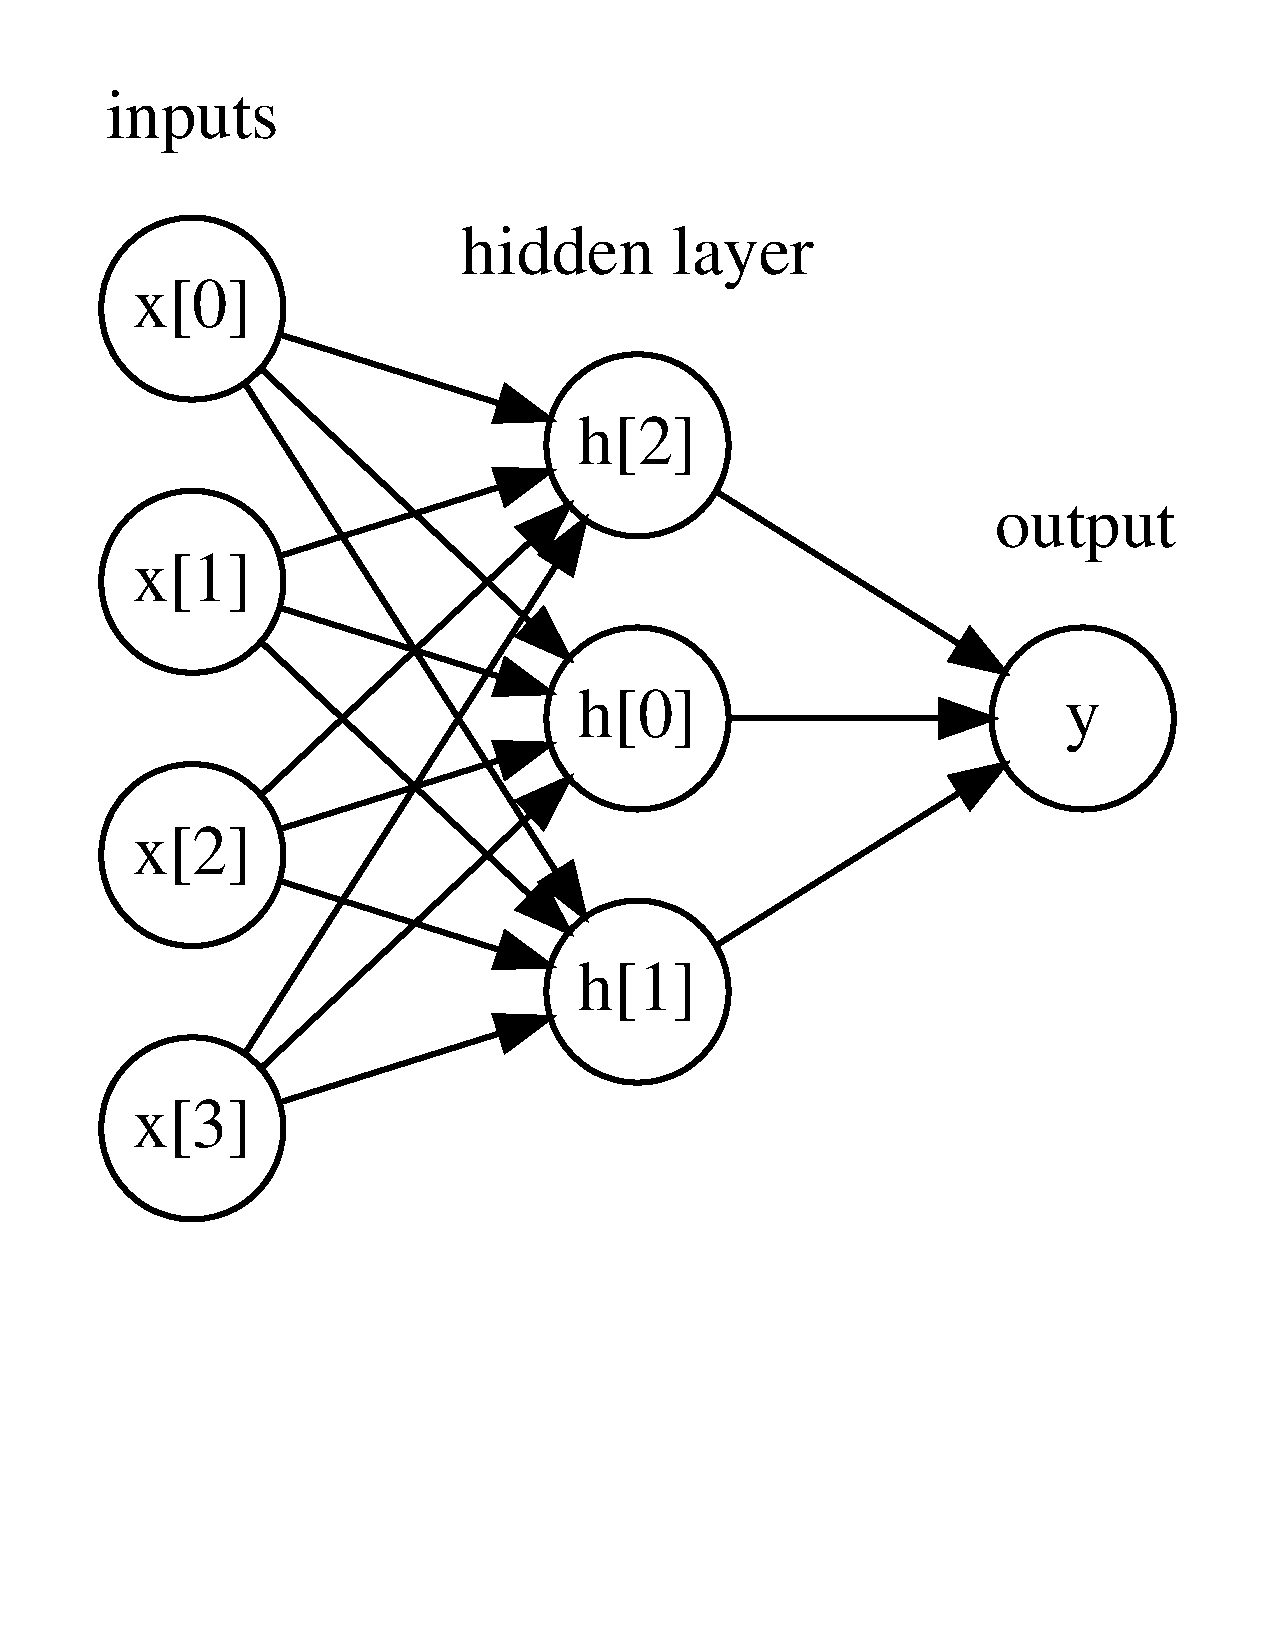
\includegraphics[page=1,width=.45\textwidth]{../Codes/Figures/Illustration of a multilayer perceptron with a single hidden layer.pdf} \\
    \end{tabular}
    \caption{Illustration of a multilayer perceptron with a single hidden layer and linear model}
    \label{Illustration of a multilayer perceptron with a single hidden layer}
\end{figure}

对于\autoref{Illustration of a multilayer perceptron with a single hidden layer}所示的小型神经网络,计算回归问题的 $\hat{y}$ 的完整公式如下(使用 tanh 非线性):

\begin{equation}
    \label{3MLP}
    \begin{split}
        h[0]    & = tanh(w[0, 0] * x[0] + w[1, 0] * x[1] + w[2, 0] * x[2] + w[3, 0] * x[3] + b[0]) \\
        h[1]    & = tanh(w[0, 0] * x[0] + w[1, 0] * x[1] + w[2, 0] * x[2] + w[3, 0] * x[3] + b[1]) \\
        h[2]    & = tanh(w[0, 0] * x[0] + w[1, 0] * x[1] + w[2, 0] * x[2] + w[3, 0] * x[3] + b[2]) \\
        \hat{y} & = v[0] * h[0] + v[1] * h[1] + v[2] * h[2] + b                                    \\
    \end{split}
\end{equation}

其中,$w$ 是输入 $x$ 与隐层 $h$ 之间的权重,$v$ 是隐层 $h$ 与输出 $\hat{y}$ 之间的权重。权重 $w$ 和 $v$ 要从数据中学习得到,$x$ 是输入特征,$\hat{y}$ 是计算得到的输出,$h$ 是计算的中间结果。需要用户设置的一个重要参数是隐层中的结点个数。对于非常小或非常简单的数据集,这个值可以小到 10;对于非常复杂的数据,这个值可以大到 10 000。也可以添加多个隐层,如图\autoref{A multilayer perceptron with two hidden layers}所示。

\begin{figure}
    \centering
    \begin{tabular}{c}
        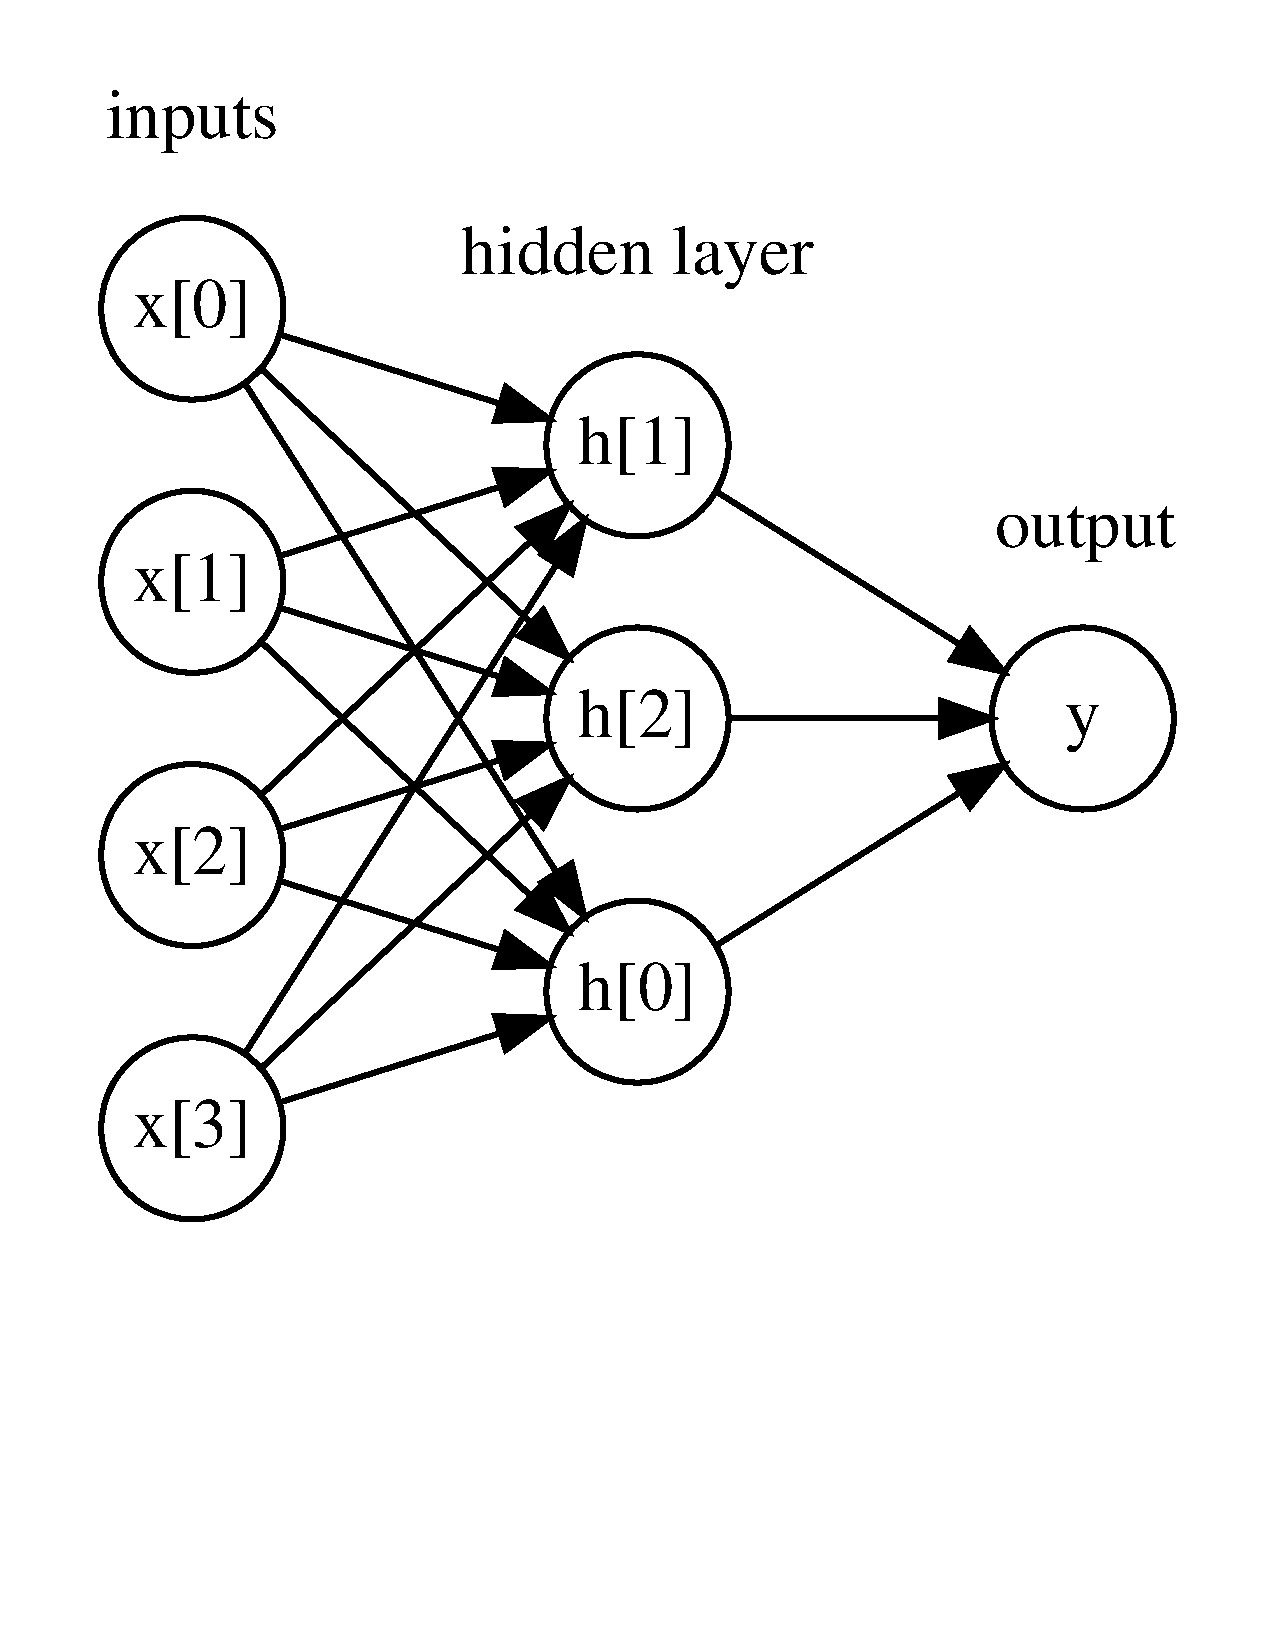
\includegraphics[page=1, width=.65\textwidth]{../Codes/Figures/A multilayer perceptron with two hidden layers.pdf} \\
    \end{tabular}
    \caption{A multilayer perceptron with two hidden layers}
    \label{A multilayer perceptron with two hidden layers}
\end{figure}

这些由许多计算层组成的大型神经网络,正是术语“深度学习”的灵感来源。

\subsubsection{神经网络调参}
将 MLPClassifier 应用到之前用过的 \verb|two_moons| 数据集上,以此研究 MLP 的工作原理。

默认情况下,MLP 使用 100 个隐结点,这对于这个小型数据集来说已经相当多了。我们可以减少其数量(从而降低了模型复杂度),但仍然得到很好的结果(图 2-49):

\autoref{3MLP}似乎有点问题,应该要写成矩阵的形式。
\subsubsection{优点、缺点和参数}
在机器学习的许多应用中,神经网络再次成为最先进的模型。它的主要优点之一是能够获取大量数据中包含的信息,并构建无比复杂的模型。给定足够的计算时间和数据,并且仔细调节参数,神经网络通常可以打败其他机器学习算法(无论是分类任务还是回归任务)。

这就引出了下面要说的缺点。神经网络——特别是功能强大的大型神经网络——通常需要很长的训练时间。它还需要仔细地预处理数据,正如我们这里所看到的。与 SVM 类似,神经网络在“均匀”数据上的性能最好,其中“均匀”是指所有特征都具有相似的含义。如果数据包含不同种类的特征,那么基于树的模型可能表现得更好。神经网络调参本身也是一门艺术。

\paragraph{估计神经网络的复杂度} 最重要的参数是层数和每层的隐单元个数。你应该首先设置 1 个或 2 个隐层,然后可以逐步增加。每个隐层的结点个数通常与输入特征个数接近,但在几千个结点时很少会多于特征个数。

神经网络调参的常用方法是,首先创建一个大到足以过拟合的网络,确保这个网络可以对任务进行学习。知道训练数据可以被学习之后,要么缩小网络,要么增大 alpha 来增强正则化,这可以提高泛化性能。

主要关注模型的定义:层数、每层的结点个数、正则化和非线性。这些内容定义了我们想要学习的模型。还有一个问题是,如何学习模型或用来学习参数的算法,这一点由 solver 参数设定。solver 有两个好用的选项。默认选项是 'adam',在大多数情况下效果都很好,但对数据的缩放相当敏感(因此,始终将数据缩放为均值为 0、方差为 1 是很重要的)。另一个选项是 'lbfgs',其鲁棒性相当好,但在大型模型或大型数据集上的时间会比较长。还有更高级的 'sgd' 选项,许多深度学习研究人员都会用到。'sgd'选项还有许多其他参数需要调节,以便获得最佳结果。当你开始使用 MLP 时,我们建议使用 'adam' 和 'lbfgs'。

\begin{tcolorbox}[title=fit 会重置模型]
    scikit-learn 模型的一个重要性质就是,调用 fit 总会重置模型之前学到的所有内容。因此,如果你在一个数据集上构建模型,然后在另一个数据集上再次调用 fit,那么模型会“忘记”从第一个数据集中学到的所有内容。你可以对一个模型多次调用 fit,其结果与在“新”模型上调用 fit 是完全相同的。
\end{tcolorbox}

\section{分类器的不确定度估计}

我们还没有谈到 scikit-learn 接口的另一个有用之处,就是分类器能够给出预测的不确定度估计。一般来说,你感兴趣的不仅是分类器会预测一个测试点属于哪个类别,还包括它对这个预测的置信程度。在实践中,不同类型的错误会在现实应用中导致非常不同的结果。想象一个用于测试癌症的医疗应用。假阳性预测可能只会让患者接受额外的测试,但假阴性预测却可能导致重病没有得到治疗。

scikit-learn 中有两个函数可用于获取分类器的不确定度估计:\verb|decision_function| 和 \verb|predict_proba|。大多数分类器(但不是全部)都至少有其中一个函数,很多分类器两个都有。
\subsection{决策函数}
\subsection{预测概率}
\verb|predict_proba| 的输出是每个类别的概率,通常比 \verb|decision_function| 的输出更容易理解。对于二分类问题,它的形状始终是 \verb|(n_samples, 2)|。

在上一个输出中可以看到,分类器对大部分点的置信程度都是相对较高的。不确定度大小实际上反映了数据依赖于模型和参数的不确定度。过拟合更强的模型可能会做出置信程度更高的预测,即使可能是错的。复杂度越低的模型通常对预测的不确定度越大。如果模型给出的不确定度符合实际情况,那么这个模型被称为\textbf{校正}(calibrated)模型。在校正模型中,如果预测有 70\% 的确定度,那么它在 70\% 的情况下正确。

\subsection{多分类问题的不确定度}

\section{小结与展望}
\begin{itemize}
    \item 最近邻:适用于小型数据集,是很好的基准模型,很容易解释。
    \item 线性模型:非常可靠的首选算法,适用于非常大的数据集,也适用于高维数据。
    \item 朴素贝叶斯:只适用于分类问题。比线性模型速度还快,适用于非常大的数据集和高维数据。精度通常要低于线性模型。
    \item 决策树:速度很快,不需要数据缩放,可以可视化,很容易解释。
    \item 随机森林:几乎总是比单棵决策树的表现要好,鲁棒性很好,非常强大。不需要数据缩放。不适用于高维稀疏数据。
    \item 梯度提升决策树:精度通常比随机森林略高。与随机森林相比,训练速度更慢,但预测速度更快,需要的内存也更少。比随机森林需要更多的参数调节。
    \item 支持向量机:对于特征含义相似的中等大小的数据集很强大。需要数据缩放,对参数敏感。
    \item 神经网络:可以构建非常复杂的模型,特别是对于大型数据集而言。对数据缩放敏感,对参数选取敏感。大型网络需要很长的训练时间。
\end{itemize}

面对新数据集,通常最好先从简单模型开始,比如线性模型、朴素贝叶斯或最近邻分类器,看能得到什么样的结果。对数据有了进一步了解之后,你可以考虑用于构建更复杂模型的算法,比如随机森林、梯度提升决策树、SVM 或神经网络。